\documentclass[12pt]{article}

\usepackage{amsmath}
\usepackage{graphicx,psfrag,epsf,amssymb}
\usepackage{enumerate}
\usepackage[top=1.0in, bottom=1.0in, left=1.0in, right=1.0in, headheight=1.0in]{geometry}
\usepackage{pdfpages} % To include activity worksheets
\usepackage{float}
\usepackage{natbib}
\usepackage{enumitem}
\usepackage{footmisc} % For footnotelayout command
\newlist{todolist}{itemize}{2}
\setlist[todolist]{label=$\square$}

\usepackage{hyperref}
\hypersetup{
    colorlinks=false,
    linkcolor=blue,
    filecolor=blue,      
    urlcolor=blue,
}

\newcommand{\blind}{0}
\newcommand{\todo}[1]{{\color{blue}[[\textbf{TODO: }#1]]}}
\newcommand{\stacey}[1]{{\color{purple}[[\textbf{Stacey says: }#1]]}}
\newcommand{\R}{\texttt{R}}

\renewcommand\footnotelayout{\fontsize{10}{12}\selectfont}

\date{December 15, 2019}

\begin{document}
\def\spacingset#1{\renewcommand{\baselinestretch}%
{#1}\small\normalsize} \spacingset{1}


%%%%%%%%%%%% DEFINING TITLE FOR PAPER & REMOVAL FOR BLIND VERSION %%%%%%%%%%%%%%

\if1\blind
{
  \title{\bf Designing Data Science Workshops for Data-Intensive Environmental 
  Science Research}
  \author{Allison Theobold \thanks{The authors gratefully acknowledge the 
  \textit{National Network of Library of Medicine}
    Data Engagement PNR grant for supporting this research.} \hspace{.2cm}\\
    Department of Statistics, California Polytechnic University \\
    San Luis Obispo, CA \\
    atheobol@calpoly.edu \\
    and \\
    Stacey Hancock \\
    Department of Mathematical Sciences, Montana State University \\
    stacey.hancock@montana.edu \\
    and \\
    Sara Mannheimer \\
    Montana State University Library \\
    sara.mannheimer@montana.edu
    }
  \maketitle 
} \fi

\if0\blind
{
  \title{\bf Designing Data Science Workshops for Data-Intensive Environmental
  Science Research}
  \author{Anonymous}
  \date{}
  \maketitle
} \fi
%%%%%%%%%%%%%%%%%%%%%%%%%%%%%%%%%

\bigskip

\begin{abstract}
% currently 182 words 

\noindent Over the last 20 years, statistics preparation has become vital for a
broad range of scientific fields, and statistics coursework has been readily 
incorporated into undergraduate and graduate programs. However, a gap remains 
between the computational skills taught in statistics service courses and those
required for the use of statistics in scientific research. Ten years after the 
publication of ``Computing in the Statistics Curriculum,'' the nature of 
statistics continues to change, and computing skills are more necessary than 
ever for modern scientific researchers. In this paper, we describe research on 
the design and implementation of a suite of data science workshops for 
environmental science graduate students, providing students with the skills 
necessary to retrieve, view, wrangle, visualize, and analyze their data using 
reproducible tools. These workshops help to bridge the gap between the computing
skills necessary for scientific research and the computing skills students 
leave their statistics service courses with. Open to faculty, staff, and the 
larger community, these workshops promote continued learning of the tools
necessary for working with data and provide additional resources for
incorporating data science into the classroom.

\end{abstract}

\noindent %
{\it Keywords:} data science, data visualization, data wrangling, \texttt{R}, 
environmental science, workshops, reproducible research 

\vfill

\newpage
\spacingset{1.45}

\section{Introduction}
\label{sec:intro}

\noindent Scientific fields have seen profound increases in the volume and variety 
of data available for analysis. Matched with the growth in computational power, 
today's scientific researchers are faced with computational and statistical 
expectations beyond the coursework dictated by their curriculum. In the
environmental sciences, though statistics courses have been readily incorporated
into undergraduate and graduate curricula, an abundance of literature suggests 
that these curricula fail to equip graduate students with the computing skills 
necessary for research in their field (Andelman et al., \citeyear{andelman}; 
Green et al., \citeyear{green}; Hampton et al., \citeyear{hampton}; Hernandez et
al., \citeyear{hernandez}, Mislan, Heer, \& White, \citeyear{mislan}; Teal et 
al., \citeyear{carpentry}; Theobold and Hancock, \citeyear{theobold}). Only 
one of these studies \citep{theobold}, however, acknowledges the substantial 
role statistics courses could potentially play in students' acquisition of 
computational skills. 

\quad Over the last 10 years, a large number of statistics educators have echoed
Nolan and Temple Lang's call to ``embrace computing and integrate it fully into 
statistics undergraduate major and graduate programs" (Nolan and Temple Lang, 
\citeyear{nolan}, p.\ 97; Baumer, \citeyear{baumer_datascience}; Baumer, Horton, 
\& Wickham, \citeyear{horton_takingachance}; Cetinkaya-Rundel and Rundel, 
\citeyear{mine}; Cobb, \citeyear{cobb}; Hardin et al., \citeyear{hardin}; Horton
and Hardin, \citeyear{horton_thinkwithdata}; Kaplan, \citeyear{kaplan}). Indeed,
the American Statistical Association's \citeyear{asa} \emph{Curriculum
Guidelines for Undergraduate Programs in Statistical Science} reflect the
increasing importance of data science skills. Despite this campaign for
computing in the statistics classroom, graduate-level statistics service courses
have largely been overlooked. Unlike courses designed for an undergraduate or
graduate program in Statistics, these service courses often act as the sole
exposure to computing with data prior to the start of a student's independent
research. A ``symptom of the current curriculum's shortcomings'' 
\citep[p.\ 547]{hampton} is the emergence of a variety of extracurricular
opportunities for acquiring critical data science skills, such as Data Carpentry
(\citeyear{data-carpentry}). While Data Carpentry's workshops teach
domain-tailored lessons covering the ``fundamental data skills'' needed for the
``full lifecycle of data-driven research,'' the possibility of tailoring these
workshops to specific populations of researchers has yet to be investigated. 

\quad The intention of this research is to (1) describe the computing skills 
necessary for graduate-level environmental science research, (2)
investigate how these skills can be infused into currently existing
extracurricular workshops, and (3) understand the experiences of attendees of
these workshops. This paper summarizes the results of the first iteration of a 
three-phase design-based implementation research model, investigating each of
these areas. For this research, the collection of disciplines who perform
research across a variety of environmental science fields are captured under the
term ``environmental science.'' At our institution, these are the departments of
Ecology, Land Resources and Environmental Sciences (LRES), Plant Sciences and
Plant Pathology (PSPP), and Animal and Range Sciences (ARS), whose students are
required or highly recommended to complete graduate-level statistics coursework
for a master's or doctoral degree. In this paper, the ``data analysis cycle''
consists of all stages in the data analysis process, from data importation to
data exploration to the communication of results (Figure \ref{fig:cycle}), where
data modeling is but one component. The ``data science skills'' necessary to
engage in this cycle may include general programming concepts such as loops,
user-defined functions, or conditional statements. However, the cornerstone of
data science skills differs fundamentally from general programming skills, with
a focus on data rather than computer architecture, design, and applications. 

\begin{figure}[h!]
    \centering
    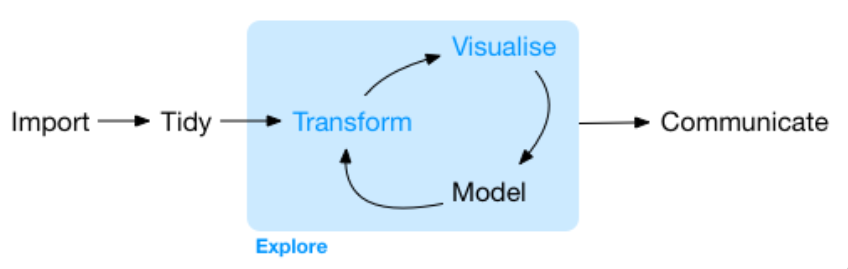
\includegraphics[width = \textwidth, height = 2in]{images/cycle.png}
    \caption{Data Analysis Cycle, Wickham, H. \& Grolemund, G. (2017) \emph{R 
    for Data Science}. Sebastopol, California: O'Reilly.}
\label{fig:cycle}
\end{figure} 

\section{The Current Climate of Statistics and Computing in the Environmental 
Sciences}
\label{sec:lit}

\noindent Due to substantial changes in the data landscape over the last twenty
years, the practice of environmental science has changed dramatically. Advances
in technology have made computationally heavy 
applications of data science techniques---such as management and coalition of 
large data sets, high frequency spatial and temporal data visualization, and 
hierarchical Bayesian modeling---essential understandings for environmental 
science research. This flood of data has ``challenged the research community's 
capacity to readily learn and implement the concepts, techniques, and tools" 
\citep[p.\ 546]{hampton} necessary for data-intensive environmental science 
research, creating a crucial need to reevaluate how our educational system can
better prepare current and future generations of researchers 
(\citeauthor{green}, \citeyear{green}; \citeauthor{hampton}, 
\citeyear{hampton}).  

\subsection{Computing in the Environmental Science Curriculum}

\noindent Arising from a decade of mumblings about the importance of computing
to environmental science research \citep{andelman, dodds1, dodds2, eglen, 
green, hastings, kelling, wilson-software-carpentry, wilson, wing}, 2012 brought
two studies on the computational ill-preparation of environmental science 
students by their curriculum. In the first large-scale study of ecology
instructors, Strasser and Hampton (\citeyear{labs}) found that undergraduate
students were not being prepared with the data management tools necessary to
engage in environmental science research. Across 51 different institutions, 
fewer than 20\% of instructors reported including data management topics in
their courses. That same year, in a survey of environmental science graduate
students across the United States, \citet{hernandez} found that over 74\%
reported they had no skills in any programming language---including 
\texttt{R}---and only 17\% reported basic skill levels in any programming
language. 

\quad Today, throughout their research, the majority of environmental science
graduate students are required to produce code as part of their data analysis
process \citep{mislan}. Dramatic changes have also been seen in the 
computing tools used in environmental science, with an increase of over 45\% in
the use of \texttt{R} in environmental science publications over the last ten 
years \citep{Rpopular}. With this changing research climate, these studies
suggest a large number of graduate students may be leaving their program without
the data science skills necessary for research in their field. Although 
statistics coursework has been readily incorporated into environmental science
degrees, these conversations have yet to acknowledge the substantial role
students' statistics education potentially plays in the attainment of the data
science skills necessary for research.

% While Hernandez and colleagues noted that student-focused workshops could
% work toward bridging this gap, by ``providing intensive environments'' where
% students could learn ``particular methods or technologies'' (p.\ 1075), 

\subsection{Computing in the Statistics Curriculum}

\noindent Changes in the digital age have also had ``a profound impact on
statistics and the nature of data analysis" \citep[p.\ 97]{nolan}, with today's
skills differing substantially from what was needed but five to ten years ago. 
In the year following the publication of ``Computing in the Statistics 
Curriculum'' \citep{nolan}, the Mckinsey Report \citep{mckinsey} was published, 
stating that, by 2018, ``the United States alone could face a
shortage of 140,000 to 190,000 people with deep analytical skills as well as 1.5
million managers and analysts with the know-how to use the analysis of big data
to make effective decisions'' (p.\ 3). With calls to transform the undergraduate
statistics curriculum, the 2014 American Statistical 
Association (ASA) President, Nathaniel Schenker, convened a workgroup to update
the association's guidelines for undergraduate programs. These new guidelines 
included an increased emphasis on data science skills and real applications, 
specifically students' ability to ``access and manipulate data in various ways,
use a variety of computational approaches to extract meaning from data, [and] 
program in higher-level languages'' \citep[p.\ 7]{asa}. 

\quad With this curricular momentum, in 2015, \emph{The American Statistician} 
produced a special issue on ``Statistics and the Undergraduate Curriculum." 
% Articles in this special issue ranged from detailing how computing should be
% included throughout the statistics curriculum \citep{jenny, tintle, hesterberg},
% to presenting thoughts on how data science topics ought to be integrated into 
% undergraduate statistics courses, \citep{esr, grimshaw, 
% baumer_datascience, hardin}.
In this issue, George Cobb (\citeyear{cobb}) provocatively stated that the
statistics curriculum needed to be rebuilt ``from the ground up,'' as ``what we
teach lags decades behind what we practice'' and ``the gap between our
half-century-old curriculum and our contemporary statistical practice continues
to widen'' (p.\ 268). Despite the issue's focus on the broader statistics
curriculum, statistics educators continued to lament that the current
Introductory Statistics curriculum teaches but a snapshot of the entire data
analysis cycle, ``wherein challenges with data computational methods, and
visualization and presentation are typically elided'' 
\citep[p.\ 336]{baumer_datascience}. 

\quad The following year brought the revised GAISE college report 
\citep{gaise}, creating a push for reform in the Introductory Statistics 
curriculum. The authors suggested two new emphases for the first recommendation
(teach statistical thinking), which better reflect the modern practice of
statistics. First, statistics educators should ``teach statistics as
an investigative process of problem-solving and decision making,'' and second,
should ``give students experience with multivariable thinking'' 
(p.\ 3). These recommendations reiterate the sentiments heard
throughout the statistics community, that students should emerge from our
courses with the understanding that data analysis ``isn't just inference and
modeling, it's also data importing, cleaning, preparation, exploration, and
visualization'' \citep{mine-jsm}. Yet, the inclusion of these topics in the
Introductory Statistics curriculum for non-majors is still a heated
discussion (Baumer et al. \citeyear{horton_takingachance}; Kaplan, 
\citeyear{kaplan}; McNamara, \citeyear{mcnamara}), as many educators believe
(1) that it is not possible to teach statistical concepts and programming in
just one course, (2) that teaching programming takes up valuable time which
could be used towards teaching important statistical concepts, or (3) students
are not interested in learning to program \citep{mine-jsm}. Thus, despite
charges for the statistics community to ``treat computing as fundamental as
basic mathematics and writing'' \citep[p.\ 298]{esr}, many students leave their
Introductory Statistics course without a set of data science skills applicable
to their lives. 

\quad The frustrations echoed by environmental science educators 
\citep{hampton, carpentry} suggest that students continue to leave the 
statistics classroom without the data science skills necessary to participate in 
the data analysis cycle. The fundamental question raised 
ten years ago by Nolan and Temple Lang still applies today: do our students
leave the statistics classroom able to ``compute confidently, reliably, and
efficiently?'' (\citeyear{nolan}, p.\ 100). An in-depth study of environmental 
science graduate students' experiences acquiring the computing knowledge
necessary for their research answered this question with a resounding `no' 
\citep{theobold}. Like the hypothesis of Teal and colleagues (2015), these
students did not attribute their data science skills to the statistics courses
they took for their degree. Rather, students gained these skills through
independent research experiences, an ``all-knowing'' past or current graduate
students, and their peer networks. Ten years after the publication of 
``Computing in the Statistics Curriculum,'' we continue to assume that 
``students will `pick up' the skills they need'' to participate in the data
analysis cycle outside of their statistics coursework \citep[p.\ 309]{gould}. 

\subsection{Extracurricular Workshops to Bridge the Gap}

\noindent Reiterated by both statistics education and environmental science 
researchers alike \citep{nolan, carpentry}, this lack of training in 
computing impedes the progress of scientific research and is 
laden with hidden costs. Students may pick up bad habits, misunderstandings, or 
the wrong concepts, learn just enough to get what they need done, spend weeks or
months on tasks that could be done in hours or days, and may be unaware of 
the reliability and reproducibility---or lack there of---of their results (Nolan
and Temple Lang, 2010, p.\ 100; Teal et al., 2015, p.\ 136). 
% But why are these
% skills still so rarely included in these statistics service courses when the
% need for them is widely recognized?

\quad Environmental science educators have restated the challenges in 
integrating computing into the curriculum outlined by Nolan and Temple Lang. 
These barriers can be boiled down to ``attempting to fit more material into
already-full courses and curriculum, which are taught by people who do not feel
prepared to address topics relevant to big data and data-intensive research'' 
\citep[p.\ 547]{hampton}. These hurdles are potentially even greater for 
graduate-level statistics service courses, where instructors are often
explicitly told the statistical content students are expected to learn, and 
implicitly assumed to also teach the data science skills necessary for students 
to participate in the entire data analysis cycle. Claiming graduate students
ought to take additional, data science-specific, courses to obtain these skills
is infeasible for many, as many graduate programs leave little room for
additional coursework. 

\quad Until computing has been meaningfully integrated into these service 
courses, extracurricular workshops hold the potential to address the gap between
the computing preparation of students by their coursework and the 
computing skills required for their research. The current drove of online
resources poses a ``significant challenge
in being able to discover relevant and high-quality materials'' 
\citep[p.\ 136]{carpentry} for researchers with limited time. Instead, short,
intensive workshops, such as those provided by The Carpentries, are able to
teach immediately useful skills that can be taught and learned quickly. As
repeated by Nolan and Temple Lang (\citeyear{esr}), extracurricular
learning opportunities are not a direct substitute for the prolonged instruction
of these skills that occurs in a course, however, this is not the goal of these
learning opportunities. Rather, workshops ``are a way to get started'' 
(p.\ 143),  lowering the activation energy required to begin acquiring computing
skills. 

% , keep learners active by using live
% coding and formative assessment, work with learners from a variety of
% backgrounds, and build learners' self efficacy \citep{null-carpentries}, so that
% attendees ``learn the computational aspects as part of an interesting,
% challenging, and confidence-building process'' \citep[p.\ 101]{nolan}.

\section{Methodology}

\noindent Improving environmental science graduate students' access to 
``powerful, effective learning opportunities'' \citep[p.\ 137]{penuel}
necessitates understanding the skills required for these students to be
successful in their research. Design-based implementation research (DBIR) 
\citep{confrey, penuel, oneill} ``offers a model for the design and testing of
innovations within the crucible of classrooms and other contexts for learning'' 
\citep[p.\ 140]{penuel}. DBIR uses collaboration with members of a
community to develop ``evidence-based improvements'' (p.\ 143) to teaching 
innovations---situating community members as ``co-designers of solutions to 
problems'' (p.\ 140) rather than bystanders. 

\quad In this article we summarize the results of the first iteration of a
three-phase DBIR model, supporting environmental science graduate students in
acquiring the data science skills necessary for data-intensive environmental 
science research. Phase one, detailed in Section \ref{sec:faculty}, focuses on
outlining the computational skills environmental science faculty members
identified as necessary for graduate students to succeed in their independent
research. Phase two of this research details how the skills identified during
phase one were used to tailor currently existing Data Carpentry 
(\citeyear{data-carpentry}) and Software Carpentry 
(\citeyear{software-carpentry}) lessons. Section \ref{sec:implement} chronicles
the third phase of this research, implementing and evaluating these workshops,
focusing on the backgrounds and experiences of workshop attendees. 

% Resources used to facilitate the
% sustainability of these workshops are outlined in Section
% \ref{sec:sustainability}, alongside possibilities for formally integrating these
% workshops into the university curricula. Finally, Section \ref{sec:future}
% outlines plans for the second iteration of this design work, and the need for
% future research investigating the learning outcomes of workshop attendees.

\quad The content of these tailored workshops was informed by the Data 
Carpentry (\citeyear {data-carpentry}) and Software Carpentry 
(\citeyear{software-carpentry}) curriculum. Adhering to the recommendations of 
the National Academies of Sciences, Engineering, and Medicine (NAS)
(\citeyear{nas}), Data Carpentry offers domain-specific curricula, so
participants ``learn more quickly and effectively,'' and can ``see more
immediately how to implement these skills and approaches in their own work''
(\citeyear{carpentry}, p.\ 136). The Data Carpentry Ecology curriculum has been
developed by the community, to ``share perspectives on best practices''
(\citeyear{carpentry}, p.\ 137). Furthermore, because these workshops are taught
numerous times across the world, with public input on the content and structure
of the lessons, the Data Carpentry Ecology curriculum represents the ``best''
theory for the teaching and learning of data science skills this field
possesses. Notably, the Carpentries does not require training for instructors
to use their content, as their materials are publicly available for use and
adaptation (with acknowledgement). 

% However, if the instructor or institution
% desires to advertise their workshops as a Carpentries sponsored workshop, the
% Carpentries requires that the lead instructor be a Carpentries certified instructor.


\section{Outlining the Computing Skills Necessary for Data-Intensive 
Environmental Science Research}
\label{sec:faculty}

\noindent As the direct supervisors of graduate students, environmental science
faculty are potentially aware of the computing skills that are vital to
researchers in their respective fields. Thus, interviews with faculty
from these fields allow for us to gain an understanding of the essential skills
required of environmental science graduate students. 

\quad In the spring of 2017 and fall of 2018, every faculty member
currently overseeing a graduate student in the Ecology, LRES, ARS, and PSPP
departments was emailed requesting their participation in this research. 
% While some faculty enthusiastically agreed to participate, others declined for
% three main reasons---they hadn't directly overseen a graduate student recently,
% they deemed themselves to be weak in statistics, or they were unavailable to
% meet. 
Table \ref{tab:faculty} outlines the number of faculty requested for
participation and the number of faculty interviewed, by departmental
affiliation. 

{\spacingset{1.05}
\begin{table}[h!]
\centering
\begin{tabular}{lcc}
\hline
Department & Faculty Invited & Faculty Interviewed  \\
\hline
Animal \& Range Sciences & 7 & 2 \\
Ecology & 15 & 8 \\
Land Resources and Environmental Sciences & 24 & 8 \\
Plant Sciences \& Plant Pathology &  15 & 5 \\ 
\hline
\end{tabular}
\caption{Number of faculty members requested for participation and interviewed,
by department.}
\label{tab:faculty}
\end{table}
}

\subsection{Data Collection \& Data Analysis}  

\noindent Faculty who agreed to participate engaged in a one-hour 
interview regarding (1) the computational skills they believe are necessary for
master's and doctoral students to implement statistics for research in their
field, and (2) how they believe graduate students acquire these necessary
skills. The full interview protocol is available as supplementary material 
\footnote{Materials associated with this manuscript are available at: anonymous 
website}.

% \href{https://github.com/atheobold/data-science-workshops-jse}{https://github.com/atheobold/data-science-workshops-jse}}

% \subsection{Data Analysis} 

\quad The primary author led a three-stage data analysis process of the faculty
interviews (Miles, Huberman, Salada$\tilde{\text{n}}$a, \citeyear{miles}). 
During the first stage, every faculty member's interviews were transcribed
verbatim. Subsequently, the primary author read each transcript, highlighting
excerpts where computing skills were discussed, creating descriptive codes for
the skills faculty identified as necessary in each of these excerpts. These
codes were then examined for references to computing
skills currently addressed in Data Carpentry's \emph{Data Analysis and
Visualization in \texttt{R} for Ecologists} lesson \citep{ecology_curriculum}. 

\quad Next, the primary author began the second stage of analytical coding,
synthesizing the descriptive codes into instances of a general concept 
\citep[p.\ 95]{miles}. During this stage, computing skills were linked
thematically, and themes that held across multiple interviews were retained.
The author then searched faculty transcripts to uncover how each theme related
to the others. During this process it was determined whether themes captured
similar constructs and should be merged, or if themes ought to remain separate. 
For example, while every faculty voiced students' need to work with data in 
\texttt{R}, these sentiments were voiced alongside students' need to perform
other data wrangling operations, such filtering out rows or selecting columns. 
Hence, the themes of ``working with data'' and ``data wrangling'' were merged
into the single theme of ``working with data.'' 

%Alternatively, while
%reproducibility is a key aspect to working with data in \texttt{R}, faculty
%sentiments regarding the need for students' work to be reproducible was not
%voiced alongside a specific software.

\quad In the final stage, the first and second authors searched the faculty
transcripts for evidence supporting the emerging themes, scrutinizing whether
each identified skill fit into the emergent themes. 
% Following this process, the first and second
% authors met to discuss the rationale for each theme and to inspect the skills
% identified by faculty in the context of the emergent themes. 
These final themes informed the design of data science workshops. 

\subsection{Themes of Skills Identified by Environmental Science Faculty}

\noindent While some faculty had difficulties disentangling the statistical methods
students use in research from the computing required to implement those methods,
many were able to express the computing skills necessary for graduate students
in their field to engage in the entire data analysis process. A substantial
overlap was seen between faculty expectations and the ``data acumen'' outlined
by NAS (\citeyear{nas}), with faculty themes falling into three categories: (1)
working with and wrangling data, (2) data visualization, and (3) reproducibilty. 

\subsubsection{Working with Data}  

\noindent Every faculty member interviewed believed that students' experiences in
the statistics classroom do not adequately prepare them to work with and
organize large, messy datasets. As graduate students perform their research,
they are required to think about ``storing data, managing data, matching
data, and collating data,'' into meaningful datasets for analysis. Some 
faculty reflected that they don't believe it's uncommon for students to work
with large datasets, but ``[they] think it's uncommon [for students] to be doing
it effectively or efficiently.'' 

\quad These skills for working with data ranged from students' ability to 
``organize their data and get it in a way that can be used by \texttt{R}'' to 
tasks that required reorganizing data formats from wide to long or vice 
versa---a skill which every faculty member griped is not acquired through the
standard curriculum. A faculty member bemoaned that standard examples in
statistics courses provide students with data which are the product
of cross-tabulation, so students are never forced ``to figure out how to get the
cross-tabulation [they] need, so that [they] can bring it into \texttt{R} and do
[their] regression.'' These concerns reiterate the importance of ``data
management and curation'' detailed by NAS, who stated that ``at the heart of
data science is the storage, preparation, and accessing of data'' 
(\citeyear[p.\ 26]{nas}). 

\subsubsection{Data Visualization} 

\noindent The importance data visualization has on every stage of students'
research was emphasized by every faculty member. Faculty affirmed
that students should possess the ability to create visualizations of their data
early and often. These expectations align with the the capabilities outlined by
NAS, who stated that students need to have the ability to ``present data in a
clear and compelling fashion'' (\citeyear[p.\ 26]{nas}). One faculty member
declared that students' ability to look at their data in different ways
dramatically shapes their research potential, and the tools available today
allow researchers to create visualizations precisely tailored for each
investigation. Many faculty voiced the usefulness of the \texttt{ggplot2} 
package \citep{ggplot} in lowering the barriers for students to learn ``how to
visualize [their] data to explore and understand it.'' 

\subsubsection{Reproducibility}  

\noindent Every faculty member emphasized the necessity for students' analysis
to be computationally reproducible, where faculty would be able to recreate 
student's results, ``given only a set of files and written instructions''
(Kitzes, Turek, Deniz, \citeyear{reproducible}). Across environmental science
disciplines, faculty concurred that many students do not perform scripted data
wrangling, and instead rely on Excel because ``[\texttt{R}] is kind of a black
box'' and when students ``don't have that instant connection with [their] data,
I think it fundamentally boils down to fear.'' Concerns were raised for the
students using unreproducible tools to wrangle their data, as ``they would never
find [their] way back to what the original data set would have been'' and their
advisers would have no way to understand why certain data are missing. While
many advisers stated that they encourage students to avoid these brute force
data manipulations, they reflected that students may not have the computing
skills necessary to perform the same tasks in a scripted and reproducible
manner. These faculty concerns parallel the ``workflow and reproducibility''
acumen outlined by NAS, who stated that students need to ``be exposed to the
concept of workflows'' (\citeyear{nas}, p.\ 28). 

\subsubsection{How Students Gain Computational Skills}

\noindent Across environmental science disciplines, faculty stated that they 
assume students are acquiring the computing skills necessary to analyze their 
data either in their required statistics coursework or on their own. When asked
why students are not acquiring computing skills in their field-specific courses,
a faculty member stated, ``we don't really have anyone to teach that. It's not
that it isn't valuable, but there is no one to teach it.'' Some faculty believed
``graduate students come in knowing more about the tools one might use to
manipulate data than their advisers do,'' while others lamented the gaps between
the computing skills of their graduate students and their own training,
feeling ``personally out of touch with [students] because I haven't taken the
time to learn \texttt{R}, because of my training and my age.'' These gaps impact
the assistance faculty can provide to their students, as ``increasingly, faculty
feel that they're not at the forefront of their programming abilities, so their
students are being self-taught and are often computationally ahead of them.''

% \quad Although faculty feel that there may exist gaps between their own
% knowledge of working in \texttt{R} and their students', every faculty member
% affirmed the importance of students acquiring the computational abilities needed
% to perform data-intensive research. Indeed, it is not necessary for every
% student to be an expert, but faculty underscored the value of resources for
% students to acquire these computational skills necessary for their research. The
% majority of faculty voiced that it is often assumed that graduate students
% should be able to analyze their data because they've taken a statistics course.
% Yet, faculty members acknowledge the poor computational preparation of their
% students---even after taking a statistics course---and thus ``encourage
% [students] to use anything they can find to get more tools in [their] tool
% box.'' 

\section{Designing Data Science Workshops for Environmental Science Graduate
Students}
\label{sec:workshops}

\noindent The second phase of this research attended to the  development of a 
suite of data science workshops targeted to graduate students in the 
environmental sciences. The skills identified through faculty interviews were
incorporated into Data Carpentry's \emph{Data Analysis and Visualization in 
\texttt{R} for Ecologists} lesson \citep{ecology_curriculum} \footnote{This
work is a derivative of \href{https://datacarpentry.org/R-ecology-lesson}{Data 
Analysis and Visualization in R for Ecologists (link)} by Data Carpentry, used
under \href{https://creativecommons.org/licenses/by/4.0/}{CC-BY License 
(link)}}. The series of workshops consists of four 3-hour workshops covering (1)
the basics of programming in \texttt{R}, (2) intermediate programming tasks in 
\texttt{R}, (3) creating effective data visualizations, and (4) wrangling data.
Importantly, the first workshop does not assume attendees have previous
experience working in \texttt{R}, and each workshop builds on the knowledge
acquired at the previous workshop(s). The workshop materials developed for this
research are available through GitHub
\footnote{Anonymous GitHub link}, 
% \href{https://github.com/atheobold/data-science-workshops-jse}{GitHub
% repository (link)}}
with video tutorials recorded and available through our institution's library  
\footnote{Anonymous YouTube link}. 
% \href{http://bit.ly/ws_recordings}{MSU Library videos (link)}}. 

% Because the
% primary author is a Carpentries certified instructor, we were able to offer the
% workshops tailored for this research as ``non-standard'' Carpentries workshops. 

\subsection{Data Context}  

\noindent Emphasized by both faculty members and NAS, ``effective
application of data science to a domain requires knowledge of that domain'' 
(\citeyear[p.\ 29]{nas}). Hence, data science instruction ought to be grounded
in ``substantive contextual examples,'' to ``ensure that data scientists develop
the capacity to pose and answer questions'' with data relevant to them
(\citeyear{nas}, p.\ 30). Therefore, ecological data are used for these
workshops, originating from a resource management agency and the
Portal Project Teaching Database \citep{portal_data}.  
%Montana Fish, Wildlife, and Parks
These data highlight a variety of aspects that
commonly occur in ecological data, including multiple sampling instances,
mark-recapture, and meta- and micro-level data. 

\subsection{Computing Tools for Environmental Science Research}  

\noindent The structure and context of these workshops include a statistical
programming language used extensively throughout environmental science research
(\texttt{R}), environments which facilitate the learning of \texttt{R}
(RStudio and RStudio Cloud), and tools that promote reproducibility throughout
the entire data analysis cycle (R Markdown).

\subsubsection{Why \texttt{R}?} 

\noindent The use of \texttt{R} is widespread throughout the environmental science
research community, a dramatic change over the last decade \citep{Rpopular}. 
Furthermore, with the creation of the RStudio integrated development 
environment (IDE) \citep{rstudio}, this user-ship continues to increase. 
% as \texttt{R} includes over 100 packages frequently used in ecological data
% analysis\footnote{\href{https://CRAN.R-project.org/view=Environmetrics}{https://CRAN.R-project.org/view=Environmetrics}}. 
\texttt{R} is free and open source, so attendees learn a statistical
programming language that will be accessible to them throughout their careers.
Unlike MARK, VORTEX, or RMAS, with \texttt{R}, attendees' results do not depend
on remembering the sequence of buttons they clicked. With a growing appreciation
for reproducible data analysis methods in ecological research 
\citep{reproducibilty-comment, repeatability, pva, reproducibility_ecology},
today's researchers in scientific fields are becoming more aware of the need for
a reproducible data analysis workflow. 

\subsubsection{Why RStudio?}

\noindent The RStudio IDE ``makes [programming] less
intimidating than the bare \texttt{R} shell" \citep[p.\ 59]{mine}. Unlike other 
statistical software packages, the RStudio environment is consistent across
operating systems. Moreover, because RStudio is an IDE, it includes integrated
help files, intelligent code completion, and syntax highlighting---all of which
help to decrease the learning curve. 

\subsubsection{Why RStudio Cloud?} 

\noindent The RStudio Cloud was created as a platform to make it easy to do,
share, teach, and learn data science using \texttt{R} \citep{RStudioCloud}. 
Through the Cloud, attendees are able to access the workshop materials without
worrying about software installation, package installation, or data transfers.
Workshop participants interact with the workshop's materials in the same manner
as a locally installed version of RStudio, as seen in Figure \ref{fig:cloud},
and are exposed to best practices for reproducible project construction through 
the use of RStudio projects. 

\begin{figure}[t!]
    \centering
    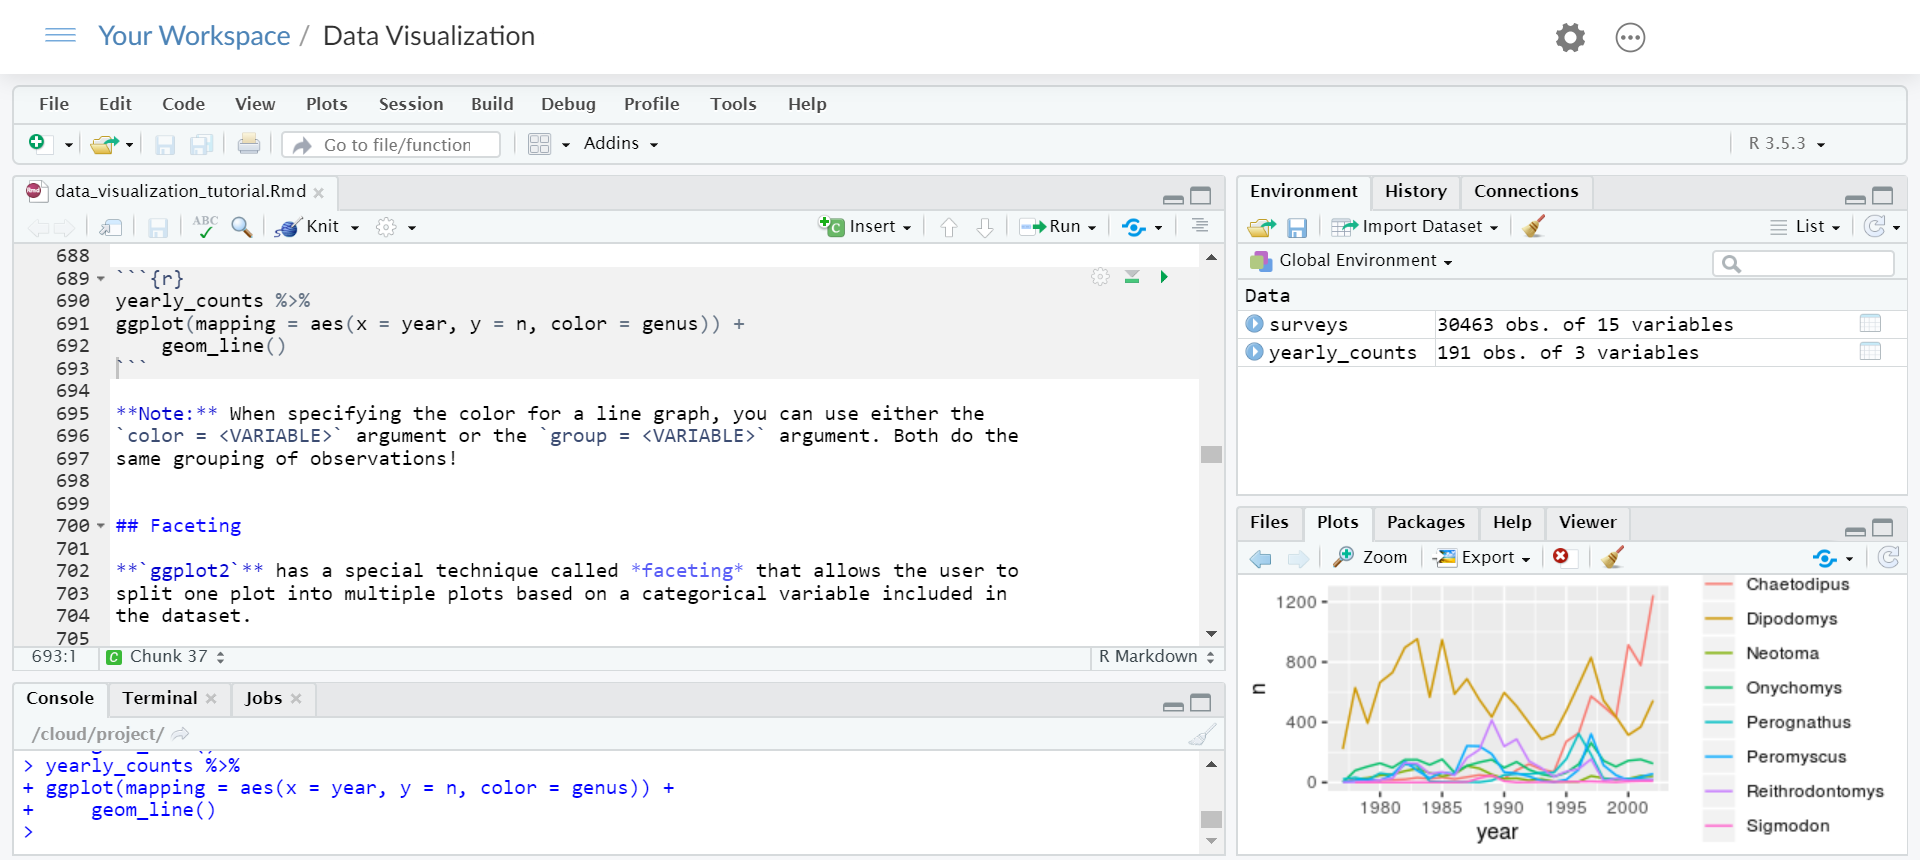
\includegraphics[width = \textwidth]{images/cloud_bigger_plot_blind.png}
    \caption{RStudio Cloud workspace environment for \emph{Data Visualization
    with \texttt{ggplot2}} workshop. Every workshop works in an RStudio project,
    containing a master R Markdown file, a data folder containing the
    data used in the workshop, and the handout produced for attendees.} 
    \label{fig:cloud}
\end{figure}

\subsubsection{Why R Markdown Documents?}

\noindent R Markdown documents provide an easy-to-understand framework to combine
statistical computing and written analysis in a single document, helping to
break the copy-paste paradigm for generating statistical reports
\citep{mine-rmarkdown}. R Markdown documents allow for attendees to keep their
code organized and their workspace clean during the workshop, a task that is 
often unnatural for new learners. For additional
information on R Markdown documents, see \citeauthor{mine-rmarkdown} 
(\citeyear{mine-rmarkdown}). 

% Each workshop's master R Markdown document
% contains blocks of code and descriptions for every topic covered, allowing for
% participants' exploratory work to be saved within a topic.

\subsubsection{Why the \texttt{tidyverse}?}

\noindent Considering much of \texttt{R}'s language has not changed over the 
last 20 years and the usage of \R~for scientific research has multiplied, there
existed a desire for a ``smoother, more efficient, and more readable pipeline
for modern \texttt{R} workflows'' (Ross, Wickham, \& Robinson, 
\citeyear{tidytools}, p.\ 19). The suite of \texttt{R} packages developed by 
Wickham and colleagues, universally known as the ``\texttt{tidyverse},'' has 
created user friendly \texttt{R} tools which ``share an underlying design
philosophy, grammar, and data structures'' \citep{tidyverse}. Inspired by how
cumbersome it can be to remember different base \texttt{R} functions to wrangle
and visualize your data, each with its own unique syntax, the workshops in this
series make use of many \texttt{tidyverse} packages, including \texttt{dplyr}
(\citeyear{dplyr}), \texttt{tidyr} (\citeyear{tidyr}), and  \texttt{ggplot2}
(\citeyear{ggplot}). The common syntax of these packages lessen learner's 
cognitive load, allowing for participants to leave each workshop with more tools
in their data science toolbox. 

\subsection{Workshop Content}

\subsubsection{Introduction to \texttt{R}}
\label{sec:introR}

\noindent This first workshop in the series covers the basics of learning to
program in \texttt{R}. The workshop first introduces the RStudio environment and
project work flow in RStudio, discussing working directories and relative paths.
Next, the workshop progresses through tools for working with vectors and lists 
of different data types, motivating methods for working with dataframes. After
learning how to import data into \texttt{R}, the workshop proceeds through
inspecting data, extracting data, and changing data types. Prompted by working
with missing data, the workshop introduces \texttt{R} help files to inspect
function arguments and their default values. These help files are called upon
as participants make use of base \texttt{R} functions to create data summaries,
perform simple data cleaning, and produce both univariate and bivariate
visualizations of the data. 

\subsubsection{Intermediate \texttt{R}}
\label{sec:intermed}

\noindent This second workshop covers coding skills to modularize \texttt{R} code. 
The content in this workshop, excluding relational statements, is not
included in Data Carpentry's \emph{Data Analysis and Visualization in \texttt{R}
for Ecologists} lesson. Yet, conditional statements, for-loops, and user-defined
functions are skills that many faculty asserted were necessary for graduate
students to possess as they perform independent research. Many of these
concepts, however, are included in Software Carpentry's 
\emph{\texttt{R} for Reproducible Scientific Analysis} lesson. 

\quad The workshop first progresses through the use of relational
statements and linking these statements using and (\texttt{\&}), or
(\texttt{|}), and not (\texttt{!}) conjunctions. Next, the workshop dives into
the use of conditional statements, stepping from \texttt{if}, to \texttt{if
else}, to \texttt{else if} statements. The second half of the workshop covers
methods to iterate or replicate a set of instructions many times. Looping,
specifically \texttt{for()} loops, are introduced as a popular way to iterate or
replicate the same set of instructions. Working through exercises which
repeat operations on a dataset using both a \texttt{for()} loop and a recursive 
\texttt{for()} loop, motivates a discussion of why vectorization is 
recommended for non-recursive \texttt{for()} loops.

\quad To conclude, functions are presented as an approach to replicate the same
set of instructions throughout your code. Inspired by a script
which copies and pastes the same process multiple times, attendees see
why this is an undesirable practice. Attendees are then tasked with transforming
the copy-paste-modify process into a function. By parsing out the function
writing process into a set of steps that should be used when you have copied and
pasted your code multiple times, participants leave with a foundational
understanding of why functions are useful and practical approaches for
implementing them in their own code.

\subsubsection{Data Wrangling with \texttt{dplyr} and \texttt{tidyr}}
\label{sec:wrangle}

\noindent The \emph{Data Wrangling} workshop introduces common data wrangling
issues faced by environmental science researchers. Using the \texttt{dplyr} 
package \citep{dplyr}, the workshop outlines six of the common ``verbs'' that
handle common data wrangling challenges: \texttt{select()}, \texttt{filter()},
\texttt{mutate()}, \texttt{group\_by()}, \texttt{summarise()}, and
\texttt{arrange()}. Prompted by the need to perform a sequence of multiple data
wrangling operations, participants learn how to connect each of these
data wrangling verbs using the pipe operator (\texttt{\%>\%}). Next, with a 
need to integrate additional data files for analysis, the concept of relational
data is outlined. After an introduction to key-value pairs, attendees
make use of the \texttt{left\_join()} and \texttt{right\_join()} functions to
join these additional data files. 

\quad The final topic of the workshop involves the issue of data reorganization.
Until now, participants have been presented with ``tidy'' data \citep{tidy}. 
% , where every
% observation is one row, each variable has a column, and every value has one
% cell. 
This concept of tidy data is used to describe `long' and `wide' data
formats. The \texttt{tidyr} package \citep{tidyr} is introduced to alleviate the
burden of data reorganizations, when transforming data from one layout to another. In
groups, participants work through a final exercise summarizing groups, using 
\texttt{pivot\_wider()} to spread these values across multiple columns, and
finally using \texttt{pivot\_longer()} to gather these multiple columns back 
together. 

\subsubsection{Data Visualization with \texttt{ggplot2}}
\label{sec:vizual} 

\noindent The final workshop in the series dives into creating data visualizations
using the \texttt{ggplot2} package \citep{ggplot}. Using the joined data from
the close of the \emph{Data Wrangling} workshop, a scatterplot is used to
illuminate a discussion of the \texttt{ggplot()} syntax. Participants learn
about the \texttt{mapping} argument
for specifying aesthetics (\texttt{aes}) for the plot and the \texttt{geom}
functions which define the type of plot you produce. By making
explicit connections between the addition operator (\texttt{+}) and the pipe
operator, participants understand addition to be an intuitive metaphor for
adding layers to a plot. Next, the workshop examines how to modify the
\texttt{ggplot()} aesthetics and geoms to create violin plots, density plots, 
bar charts, and line plots, allowing for participants to explore the 
\texttt{geom} functions and aesthetics that pair with each plot. A conversation
is had about the importance of plotting raw data rather than simply aggregate
measures of the data, and the difficulties that might arise. Adding a
\texttt{geom\_point()} or \texttt{geom\_jitter()} layer to a visualization
highlights tools that can be used so graph elements don't interfere with the
data (e.g. jittering, transparency), similar to the advice of Nolan and Perrett
(\citeyear{nolan-viz}). Finally, faceting, using \texttt{facet\_wrap()} and
\texttt{facet\_grid()}, is introduced as an additional visualization tool to
facilitate multivariate comparisons \citep[p.\ 261]{nolan-viz}. 

\quad By this point in the workshop, participants have posed many questions on
how to modify aspects of a plot that don't depend on the geom. For the final 
section of the workshop, the group walks through different customizations one 
can make to each \texttt{ggplot} object to add clarity and information to the 
plot. Participants learn how to flip a plot's coordinates, and how to make
customizations of the labels, the size of the points, the thickness of
lines, the appearance of the plotting window, and the colors. Each of
these customizations continues to emphasize the iterative nature 
of creating data visualizations, transforming a simple plot step-by-step ``into
a graph that is data rich and presents a clear vision of the important features
of the data'' \citep[p.\ 262]{nolan-viz}.

\section{Evaluating Data Science Workshops}
\label{sec:implement}

\noindent During the 2018-2019 academic year, a total of 202 students, faculty,
and staff attended at least one workshop. The \emph{Introduction to \R} and
\emph{Intermediate \R} workshops were offered twice during the fall semester,
and once during the spring semester, with 84 individuals attending 
\emph{Introduction to \R} and 74 attending \emph{Intermediate \R}. The 
\emph{Data Wrangling} and \emph{Data Visualization} workshops were each offered
once during the spring semester, with a total of 20 individuals attending 
\emph{Data Wrangling} and 24 attending \emph{Data Visualization}. The first
workshop was offered two weeks after the start of the semester, with three week
breaks between each subsequent workshop. 
% Each workshop lasted three hours and
% was taught by one lead instructor with two workshop assistants. 

\quad In the week prior to each workshop, a survey was
sent out using a Google Form. This survey detailed individuals' demographics and
backgrounds prior to attending the workshop. Following each workshop, attendees
were asked to complete a survey, detailing their experiences in
the workshop. The submission of these surveys requires responses to every
question. The content of these surveys was informed from the assessments 
developed by The Carpentries \footnote{This work is a
derivative of The Carpentries \href{https://carpentries.org/assessment/}{pre-
and post-workshop survey materials (link)}, used under 
\href{https://creativecommons.org/licenses/by/4.0/}{CC-BY License (link)}, with
revisions to disciplines and occupations, and removal of questions regarding
frequency of use of computing tools and the level of agreement with provided
statements}. Of the 202 students, faculty, and staff that attended these
workshops, 121 (60\%) completed the pre-workshop survey and 56 (27\%) completed
the post-workshop survey. The pre- and post-workshop surveys are available
through GitHub \footnote{Anonymous GitHub link}.
% \href{https://github.com/atheobold/data-science-workshops-jse}{GitHub
% repository (link)}}


\subsection{Backgrounds of Workshop Participants}

\noindent The majority of the workshop attendees were from environmental science
fields---from departments such as LRES, Ecology, PSPP, Biochemistry or
Microbiology, ARS, and Earth Sciences. Over 60\% of workshop attendees were
master's and doctoral students. It is worth noting, however, that 18 faculty,
staff, and postdocs also attended these workshops. Figure \ref{fig:departments}
displays the department affiliations of the workshop attendees and their
reported occupation. 

{\spacingset{1.05}
\begin{figure}[h!]
\centering
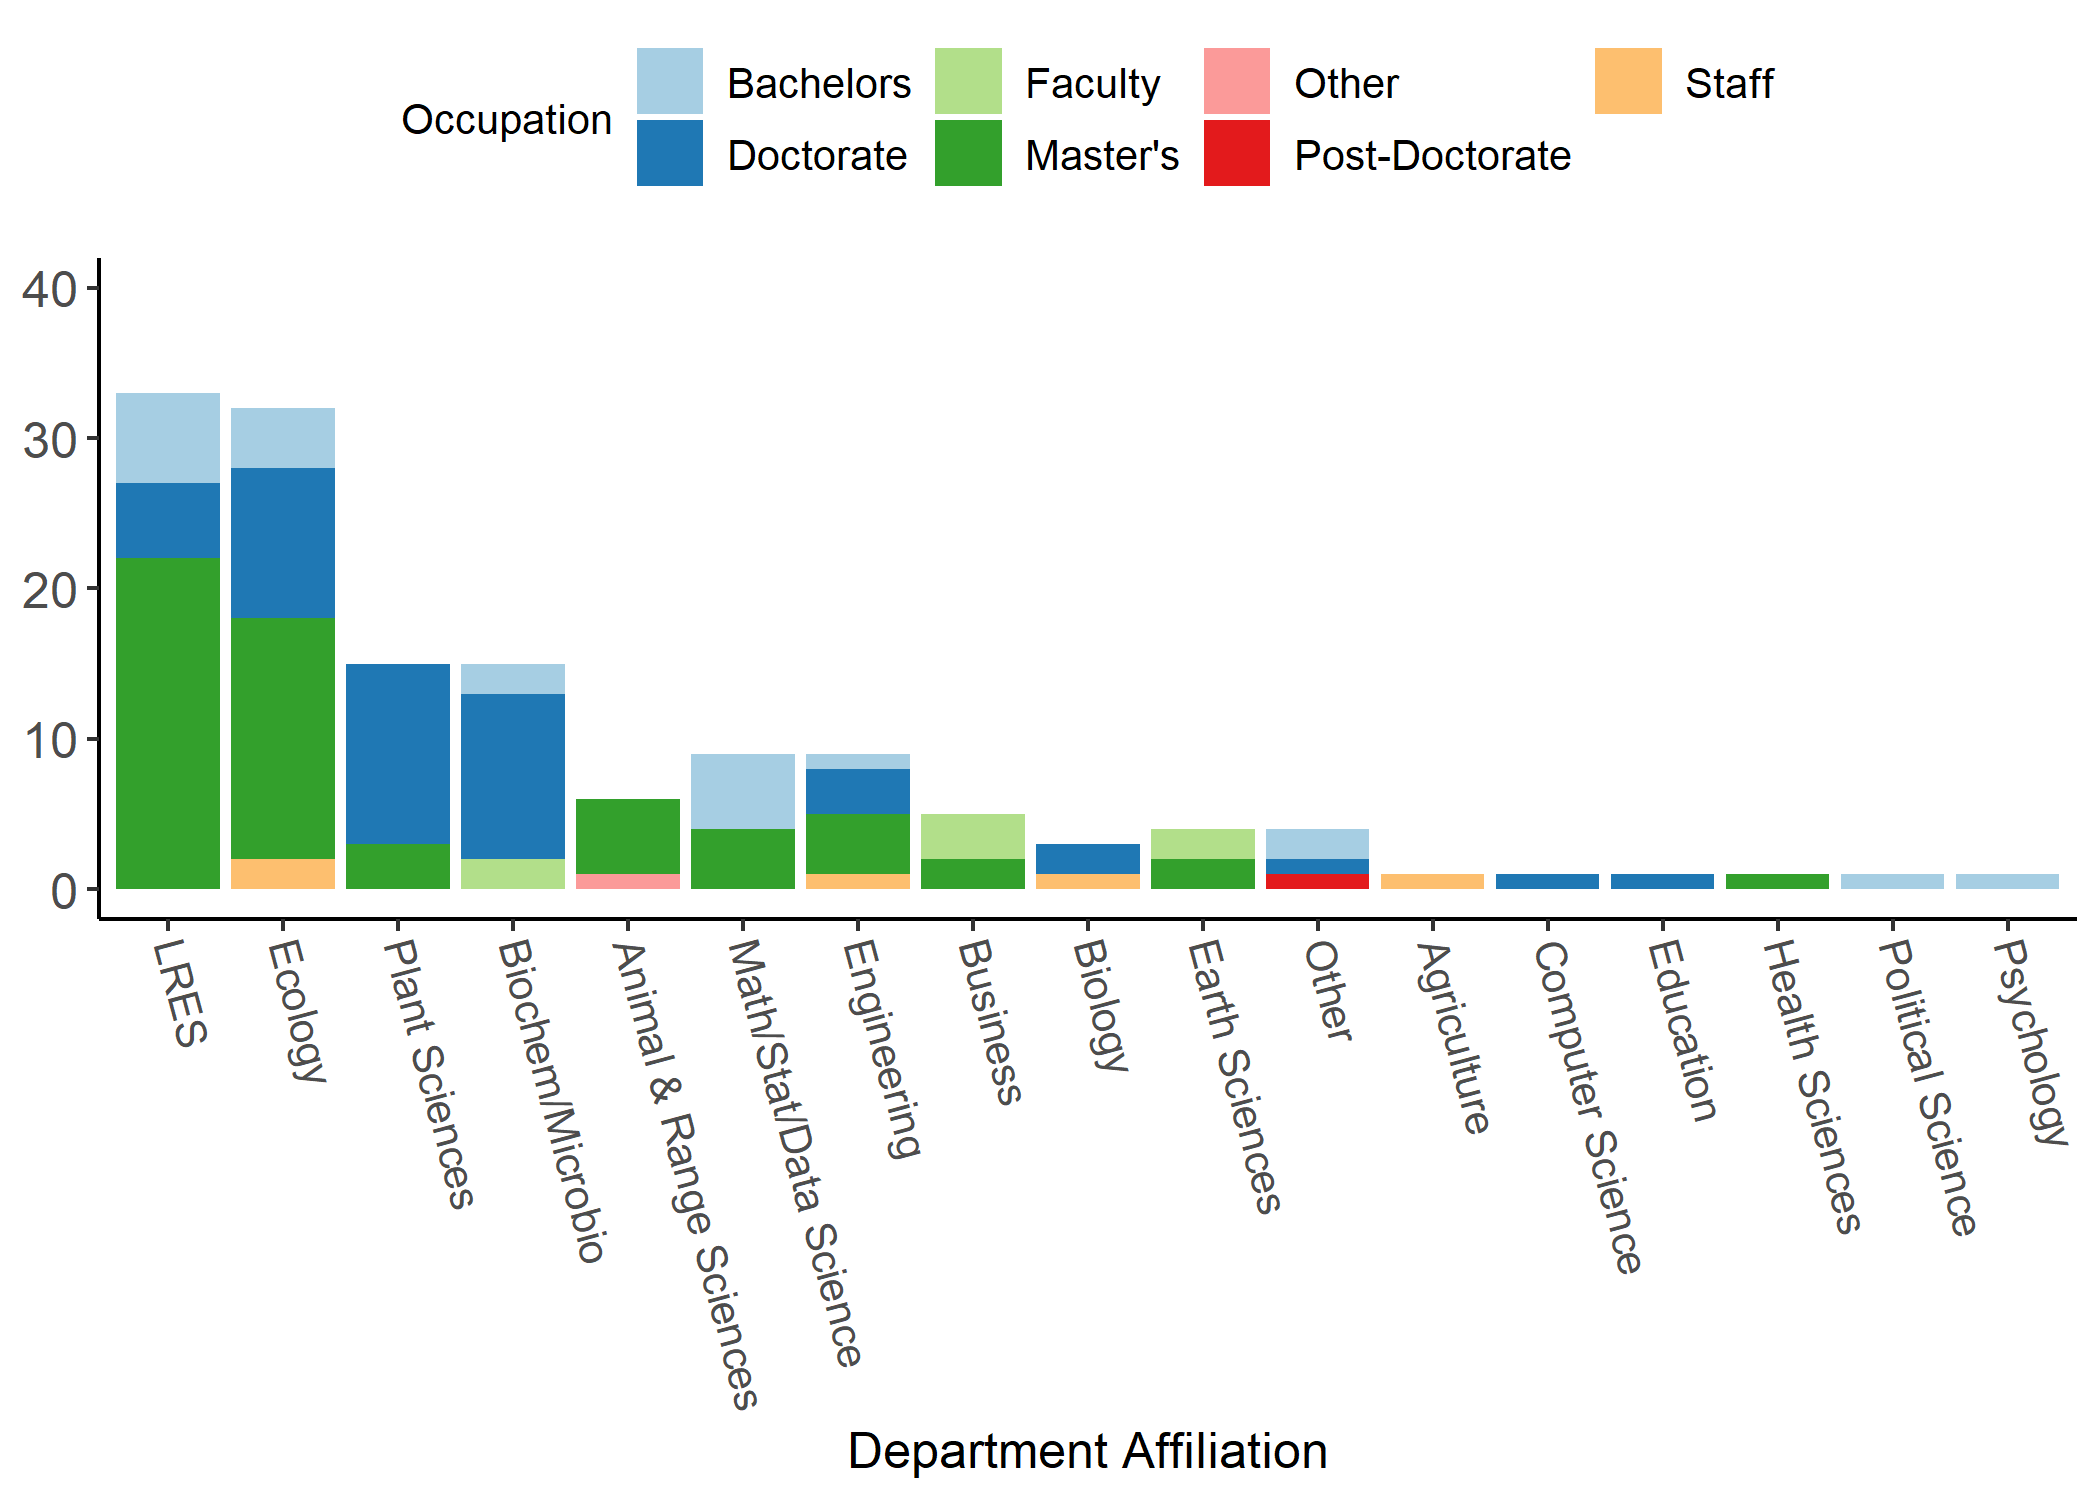
\includegraphics[width = \textwidth]{images/better_colors_attendance.png}
\caption{Number of workshop attendees during the 2018-2019 academic year, by
department and current occupation, selected from an itemized list of campus
departments and positions in the pre-workshop survey.}
    \label{fig:departments}
\end{figure}
}

\quad Consistent with the environmental science literature \citep{andelman, 
hampton, hernandez, carpentry}, the majority of attendees (over 60\%) reported
no experiences with any programming languages. However, 20\% of attendees 
reported experiences working in \texttt{R}, and 30\% reported experiences with
other programming languages (e.g., MatLab, SQL, Java, C). 

\quad Many attendees, however, stated that they had taken courses in statistics, 
with the majority reporting undergraduate or graduate experiences in an
introductory level statistics course. Most graduate students had taken 
discipline-specific introductory statistics courses in their own department or
a graduate-level applied statistics course offered by the Department of
Mathematical Sciences. Table \ref{tab:statistics} consolidates workshop
participants' previous statistical experiences. Notably, over 15\% of
attendees reported having no formal statistical training. 

{\spacingset{1.05}
\begin{table}[h!]
    \centering
    \begin{tabular}{lc}
\hline
Stat Courses & Participants \\
\hline
Introductory Statistics & 46 \\
Applied Statistics & 42 \\
None & 24 \\
Discipline Specific Introductory Statistics & 20 \\
Intermediate Statistics & 10 \\
Experimental Design	& 8 \\
Probability Theory	& 6 \\
Statistical Computing & 3 \\
Sampling & 3 \\
Biostatistics & 2 \\
Spatial Analysis & 2 \\
Econometrics & 1 \\
Time Series Analysis & 1 \\
\hline
\end{tabular}
\caption{Workshop attendees' responses (n = 121) to the pre-workshop survey
question ``What are your previous statistical experience(s)?  List course
names.,'' thematically organized based on content of the course.}
\label{tab:statistics}
\end{table}
}

\subsection{Motivation for Attending} 

\noindent As expected from the prevalence of the use of \texttt{R} in environmental
science research \citep{Rpopular, mislan}, over half of the master's, doctoral, 
and post-doc workshop participants attended the workshop for research
assistance. Other attendees were seeking assistance with learning the \R~skills
necessary for their coursework, refreshing or updating their \texttt{R}
skills to include new tools they were unfamiliar with (e.g. \texttt{ggplot}, 
\texttt{dplyr}), or undergraduates preparing for graduate school. As echoed by
previous studies of environmental science graduate students \citep{carpentry,
theobold}, attendees overwhelmingly stated that they primarily use the internet
(27\%), their peers (21\%), or their lab mates (15\%) when learning \texttt{R}.

% Based on the statistical backgrounds of these
% participants and the statistics education literature on computing in the
% statistics classroom, it is not surprising that nearly two-thirds of these 
% individuals reported using resources other than course materials as their main 
% resource for learning \texttt{R}. 

\subsection{Reflections of Workshop Participants} 

\noindent The percentage of individuals reporting the workshop covered 
unfamiliar material differed by workshop, with 40\% of \emph{Introduction
to \texttt{R}} participants, 30\% of \emph{Intermediate \texttt{R}}
participants, 80\% of \emph{Data Wrangling} participants, and 50\% of 
\emph{Data Visualization} participants stating the information presented was
new to them. Across every workshop, nearly every participant stated that they
``strongly agreed'' that they ``learned skills that [they] will be able to use
in [their] research/work.'' Additionally, over 75\% of the workshop participants
reported they would use the skills they learned in their research immediately or
in the next 30 days. 

\quad Themes of hands-on learning, workshop atmosphere, instructor attributes,
and confidence emerged from attendees' reflections of what they enjoyed most
about the workshop. Many attendees felt the hands-on exercises ``foster[ed] a
much greater level of understanding,'' left them feeling more ``confident
figuring things out on my own,'' and were ``a clear tool which allow me to see
what I gained.'' Furthermore, these attendees voiced that the workshop left them
feeling more independent, because ``I have a better understanding of how to read
code, what certain symbols/terms/etc mean and how they work.'' 

\section{Sustainability of Workshops}  
\label{sec:sustainability}

\noindent To facilitate the sustainability of these workshops, we forged a
partnership between our institution's library and the Department of Mathematical
Science's Statistical Consulting and Research Services (SCRS). We believe a 
university's library is an optimal unit for offering these workshops, as it is
both department-agnostic and a central hub for the entire university community.
Furthermore, by partnering with an organization that provides statistical
consulting, workshop participants are provided with a potential avenue if
difficulties or additional questions arise---so the peer network is not shifted 
onto workshop instructors. 

\quad A data-engagement grant from the National Network of Libraries of Medicine
during the 2018-2019 academic year supported the primary author in leading the
workshops, becoming a Carpentries certified instructor, and incorporating the
results of this research into the broader Data and Software Carpentry curricula.
A \$5,000 faculty excellence grant during the 2019-2020 academic year,
facilitated the implementation of a ``train-the-trainer'' model, training two 
future graduate student instructors. Students were recruited from the Master's
and Doctoral programs in Statistics, but because of the widespread use of 
\texttt{R} across scientific fields, students from a variety of backgrounds hold
the potential to be effective instructors. Both semesters, the authors met with 
these students for one hour a week to build students' facilities and confidence
instructing. Each semester, students taught different 30 to 45 minute portions
of each workshop, and acted as assistants for the remainder for the workshop.  

% \quad Currently, this design research is focusing on incorporating the content of these workshops into the \emph{Data Analysis and Visualization in \texttt{R}} lesson within Data Carpentry's Ecology curriculum. Infusing the skills outlined in this research into the \emph{Data Analysis and Visualization in \texttt{R} for Ecologists} lesson helps to create a Carpentries curriculum that best reflects the ``core data skills'' necessary for data-intensive environmental science research. For skills outlined by this research where there is no room in the current \emph{Data Analysis and Visualization in \texttt{R} for Ecologists} lesson, the Carpentries Incubator and Carpentries Lab provide potential avenues to produce additional lesson materials that are broadly available to The Carpentries community. These avenues allow for the continued discussion of the importance of integrating user-defined functions, conditional statements, and loops into the broader Data Carpentry Ecology curriculum.    

\quad Similar to the Explorations in Statistics Research workshop model
\citep{esr}, the ``standard'' Carpentries workshop format takes place over an
intensive two days. Self-organized workshops, however, allow for this format to
tailored to be more conducive for busy students, faculty, and staff, but this
revised format has both benefits and costs. The additional time between each
workshop helps to alleviate the fatigue often experienced in intensive
workshops, and allows for participants to selectively attend workshops relevant
to the skills they wish to acquire. However, in this extended format, workshops
after \emph{Introduction to \texttt{R}} are potentially
considered ``specialized'' workshops and experience lower attendance. At an
academic institution, there is the possibility of integrating this type of
workshop series into a single credit course. When considering this as an option,
however, institutions should think carefully about how faculty and staff can 
continue to participate in these learning opportunities. Alternatively,
institutions could offer course credit for undergraduate students assisting with 
the workshops, and allow for students to become lead or co-instructors as they
progress through their program.

\section{Limitations \& Future Research} 
\label{sec:future}

\noindent The sentiments heard by faculty in this research unearth the
possibility that many faculty may be unaware of the computing skills necessary
for their graduate students to participate in the entire data analysis cycle.
Instead, students may have more relevant knowledge regarding the data science
skills that are necessary for their research. Hence, the next iteration of this
research will focus on the collection of the \texttt{R} code produced
by environmental science graduate students throughout their research. The skills
outlined by this research aid in reevaluating the content of these workshops, to
ensure they cover the skills necessary for graduate-level environmental science
research. 

% Graduate students' research
% code acts as artifacts of their research experience, providing ``mute evidence''
% \citep{hodder} of the data science skills necessary throughout their data
% analysis cycle. 

\quad The attendance of these tailored workshops by students,
faculty, and staff from disciplines outside of environmental science brings
to question whether these types of discipline-specific workshops are necessary.
Over a third of the workshop attendees came from disciplines outside of 
environmental science, and, strikingly, these attendees reported similar
workshop experiences to attendees from these targeted disciplines. This brings
to question if there are common computational understandings necessary for
research in \emph{any} scientific field, which should be infused into 
\emph{every} statistics and data science course. Alternatively, we saw a greater
persistence across workshops by attendees from environmental science fields. 
This causes us wonder, what are the drivers behind these individuals' continued
attendance? Future research investigating the learning outcomes of workshop
attendees holds the potential to provide fruitful insight into the necessity of
discipline-specific learning opportunities. 

% Research on drift/questions in WS
% \quad Finally, despite the increasing availability of extracurricular 
% workshops, research has yet to investigate the consistency or drift of these 
% workshops. In this research, because of the large attendance at many
% \emph{Introduction to \texttt{R}} workshops, a large number of questions would
% arise over the course of the afternoon. This lead to an inability to cover some
% of the workshop content in as much depth as hoped, yet some attendees remarked 
% that ``with so many people, [the workshop] had better discussions.'' A large 
% scale analysis of the content covered by these workshops could unearth common
% questions or misunderstandings, aiding in the reconstruction of lessons to
% better scaffold learning. 

\section{Conclusion}
\label{sec:conclusion}

\noindent Ten years ago, Nolan and Temple Lang declared that ``modernizing the
statistics curricula to include computing [...] is an issue that deserves
widespread attention and action'' (p.\ 106). Over the last ten years, we have
seen both small and large changes advocated for the statistics curriculum. 
However, graduate-level statistics service courses have received less
attention and pose different issues. 

\quad Statistics courses that serve a variety of students (undergraduate,
graduate, statistics major, non-major) reflect a snapshot of the statistics
curriculum, and often act as many students' sole statistics course prior to
conducting scientific research. Instructors of these courses thus grapple with 
difficult decisions of how they can ensure their students have both the
statistical and ``computational understanding, skills, and confidence needed to
actively and wholeheartedly participate'' in the scientific research arena 
\citep[p.\ 106]{nolan}. For instructors unfamiliar with students' scientific
disciplines, it can be difficult to ``be bold and design curricula from
scratch'' (p.\ 106). The topics suggested by Nolan and Temple Lang
(2010) represent a starting point toward building a taxonomy for computing in
statistics for undergraduate and graduate Statistics programs. These topics,
however, may not be relevant to or emphasized by other scientific disciplines
whose students enroll in statistics service courses.  In our
research, we found that environmental science faculty stressed the importance of
graduate students developing skills surrounding the fundamentals of working with
data in \texttt{R}, wrangling skills for data processing and preparation, 
creation of data visualizations, and usage of reproducible work flows. 

\quad The time is ripe for us to ``update the foundational concepts and
infrastructure'' \citep[p.\ 5]{crossroads} included in statistics service
courses, in the new era of data science. As we work toward a more thorough
integration of computing into these courses, this research offers a model for
facilitating external workshops, which hold the potential to fill a critical
hole in the curriculum of many college programs. External workshops allow for 
co-curricular learning, when paired with statistics service courses, so students
leave their statistics course with the computing skills necessary to engage in
the entire data analysis cycle. Moreover, these workshops support
university-wide data science literacy, facilitating avenues for faculty to
acquire data science knowledge and skills which ``they have not had the
opportunity to learn well'' \citep[p.\ 106]{nolan}, and providing resources for
instructors to meaningfully integrate discipline-specific computing skills into
their classroom. 

% Additionally, because workshops are able to thrive outside of university
% curricula, they hold the ability to ``adapt materials rapidly and remain on the
% leading edge of technological development'' \citep[p.\ 547]{hampton}.
% Furthermore, workshops offer the opportunity for a wide variety of researchers,
% not just students, to acquire the data science skills necessary for
% data-intensive research, supporting the broader community of researchers. 

% This collaboration 
% is critical when developing resources for researchers in the broader scientific
% community, as the discipline of Statistics was developed to support research in
% other scientific disciplines to evaluate evidence obtained from data. 

\section{Acknowledgements}

\noindent We would like to specially thank the participants of this study,
without whom this research would not have been possible. We would also like to
thank the workshop instructors and helpers for helping to grow the data
literacy across our campus. Finally, thanks to Jennifer Green, Mark Greenwood,
Johanna Hardin, and the reviewers for their insightful comments.  

\bibliography{ref}
\bibliographystyle{apalike}

\end{document}
